%Talk given virtually for SIAM UQ 2020 March
\documentclass[10pt,compress,xcolor={usenames,dvipsnames},aspectratio=169]{beamer}
%\documentclass[xcolor={usenames,dvipsnames},aspectratio=169]{beamer} %slides and 
%notes
\usepackage{amsmath,
	amssymb,
	datetime,
	mathtools,
	bbm,
	%mathabx,
	array,
	booktabs,
	xspace,
	multirow,
	calc,
	colortbl,
	siunitx,
 	graphicx}
\usepackage[usenames]{xcolor}
\usepackage[giveninits=false,backend=biber,style=nature, maxcitenames =10, mincitenames=9]{biblatex}
\addbibresource{FJHown23.bib}
\addbibresource{FJH23.bib}
\usepackage{newpxtext}
\usepackage[euler-digits,euler-hat-accent]{eulervm}
\usepackage{media9}
\usepackage[autolinebreaks]{mcode}
\usepackage[tikz]{mdframed}


\usetheme{FJHSlimNoFoot169}
\setlength{\parskip}{2ex}
\setlength{\arraycolsep}{0.5ex}

%\renewcommand{\qedsymbol}{}

\DeclareMathOperator{\INT}{INT}
\DeclareMathOperator{\AVG}{AVG}
\DeclareMathOperator{\sol}{SOL}
\DeclareMathOperator{\app}{APP}
\DeclareMathOperator{\alg}{ALG}
\DeclareMathOperator{\ACQ}{ACQ}
\DeclareMathOperator{\ERR}{ERR}
\DeclareMathOperator{\COST}{COST}
\DeclareMathOperator{\COMP}{COMP}
\DeclareMathOperator{\LIN}{LINEAR}
\DeclareMathOperator{\BAD}{BAD}
\newcommand{\dataN}{\bigl(\hf(\vk_i)\bigr)_{i=1}^n}
\newcommand{\dataNj}{\bigl(\hf(\vk_i)\bigr)_{i=1}^{n_j}}
\newcommand{\dataNjd}{\bigl(\hf(\vk_i)\bigr)_{i=1}^{n_{j^\dagger}}}
\newcommand{\ERRN}{\ERR\bigl(\dataN,n\bigr)}

\newcommand{\Sapp}{S_{\textup{app}}}
\newcommand{\LambdaStd}{\Lambda^{\textup{std}}}
\newcommand{\LambdaSer}{\Lambda^{\textup{ser}}}
\newcommand{\LambdaAll}{\Lambda^{\textup{all}}}
\newcommand{\oton}{1\!:\!n}
\newcommand{\talert}[1]{\alert{\text{#1}}}
\DeclareMathOperator{\init}{init}
\DeclareMathOperator{\GP}{\cg\cp}
\newcommand{\MLE}{\textup{EB}}
\newcommand{\mCtheta}{{\mathsf{C}_{\vtheta}}}
\newcommand{\mCInv}{\mathsf{C}^{-1}}
\newcommand{\tvg}{\widetilde{\vg}}

%\DeclareMathOperator{\app}{app}

\providecommand{\HickernellFJ}{H.\xspace}


\iffalse

\fi

\renewcommand{\OffTitleLength}{-7ex}
\setlength{\FJHThankYouMessageOffset}{-8ex}
\title{The Reisz Representation Theorem}
\author[]{Fred J. Hickernell}
\institute{Department of Applied Mathematics \&
	Center for Interdisciplinary Scientific Computation \\  Illinois Institute of Technology \quad
	\href{mailto:hickernell@iit.edu}{\url{hickernell@iit.edu}} \quad
	\href{http://mypages.iit.edu/~hickernell}{\url{mypages.iit.edu/~hickernell}}}

\thanksnote{Thanks to the Illinois Tech Student Chapter for the invitation}
	
\event{My Favorite Theorem}
\date[]{October 19, 2021}

\input FJHDef.tex


\newlength{\figwidth}
\setlength{\figwidth}{0.25\textwidth}

\newlength{\figwidthSmall}
\setlength{\figwidthSmall}{0.2\textwidth}

\newcommand{\financePict}{\href{http://i2.cdn.turner.com/money/dam/assets/130611131918-chicago-board-options-exchange-1024x576.jpg}{\includegraphics[width
		= 3cm]{ProgramsImages/130611131918-chicago-board-options-exchange-1024x576.jpg}}}
	
	\newcommand{\scoop}[1]{\parbox{#1}{
\includegraphics[width=#1]{IceCreamScoop.eps}}\xspace}
	\newcommand{\smallscoop}{\scoop{1cm}}
	\newcommand{\medscoop}{\scoop{1.8cm}}
	\newcommand{\largescoop}{\scoop{3cm}}
	\newcommand{\ICcone}[1]{\parbox{#1}{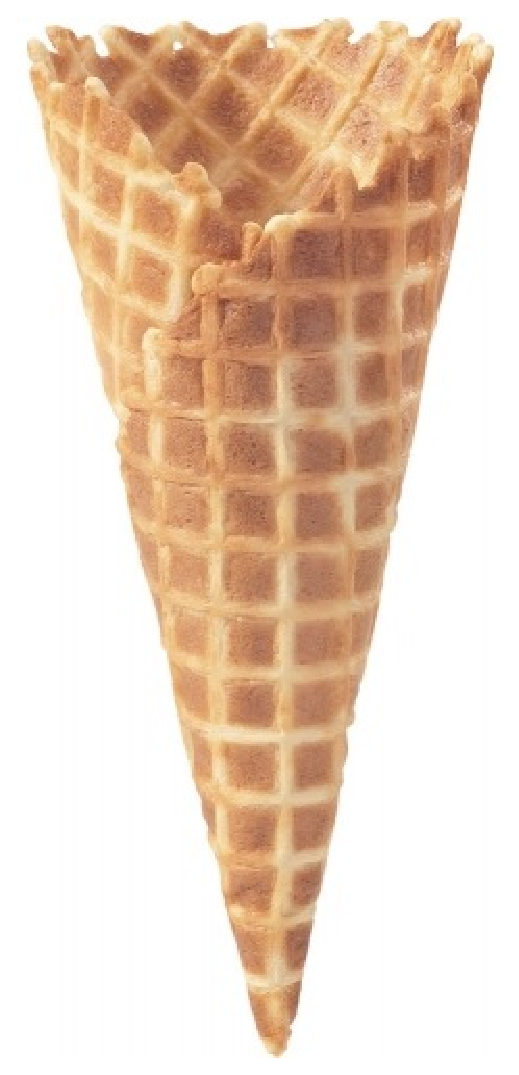
\includegraphics[width=#1,angle=270]{MediumWaffleCone.eps}}\xspace}
	\newcommand{\medcone}{\ICcone{1.2cm}}
	\newcommand{\largercone}{\parbox{2.2cm}{\vspace*{-0.2cm}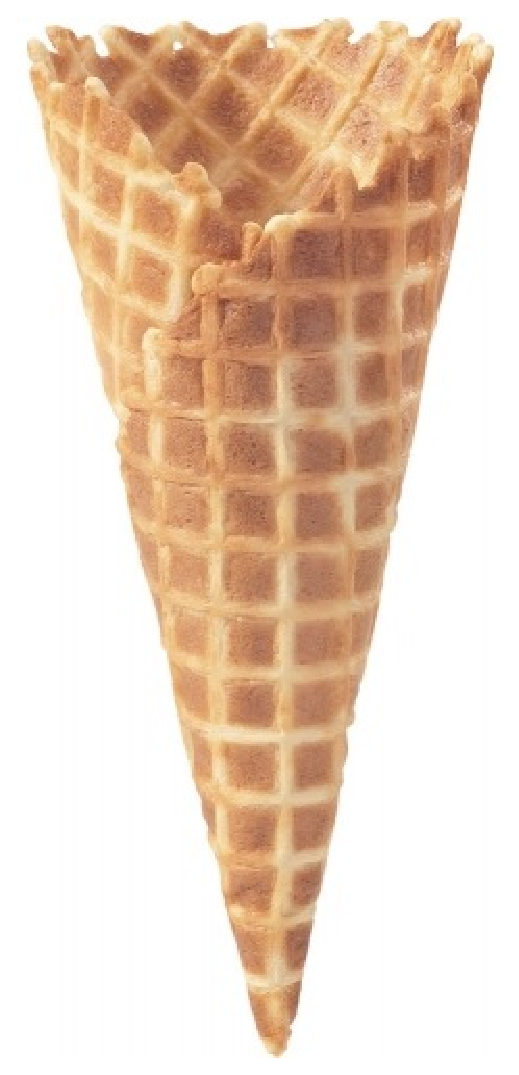
\includegraphics[width=1cm,angle=270]{MediumWaffleCone.eps}}\xspace}
	\newcommand{\largecone}{\ICcone{1.8cm}}
	\newcommand{\smallcone}{\parbox{1.1cm}{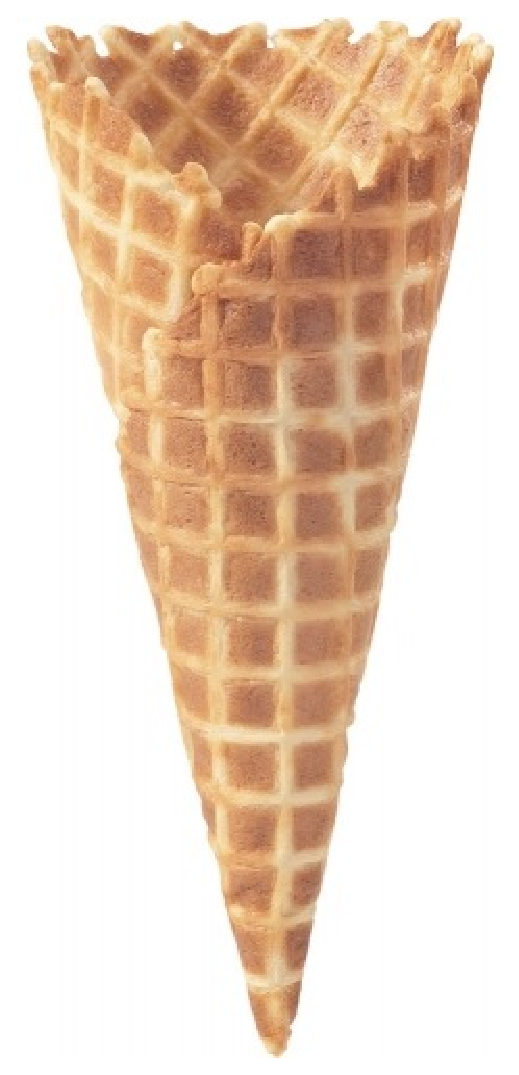
\includegraphics[width=0.5cm,angle=270]{MediumWaffleCone.eps}}\xspace}

	

\newcommand{\northeaststuff}[3]{
	\begin{tikzpicture}[remember picture, overlay]
	\node [shift={(-#1 cm,-#2 cm)}]  at (current page.north east){#3};
	\end{tikzpicture}}


\begin{document}
	\tikzstyle{every picture}+=[remember picture]
	\everymath{\displaystyle}

\frame{\titlepage}

%%%%%%%%%%%%%%%%%%%%%%%%%%%%%%%%%%%%%%%%%%
%%%%%%%%%%%%%%%%%%%%%%%%%%%%%%%%%%%%%%%%%%
\section{Background}
%%%%%%%%%%%%%%%%%%%%%%%%%%%%%%%%%%%%%%%%%%
%%%%%%%%%%%%%%%%%%%%%%%%%%%%%%%%%%%%%%%%%%

\begin{frame}{Main Idea}
    What seems \alert{obvious} for $d$-dimensional vectors becomes a power tool for \alert{numerical analysis}
    
    \begin{description}
    \item[Obvious]<2-> If $\LIN: \reals^2 \to \reals$ is any \alert{linear, real-valued} function, \uncover<2-4>{meaning,
    \[
    \LIN(c\vf + \vh) = c \LIN(\vf) + \LIN(\vh) \qquad \forall \vf, \vh \in \reals^3, \ c \in \reals,
    \]}
    then we can represent $\LIN(f)$ as an \alert{inner product}\uncover<2-4>{:
    \[
    \LIN(\vf) = g_1 f_1 + g_2 f_2 = \vg^T \vf =: \ip{\vg}{\vf} \equiv \vg \bigcdot \vf \quad \forall \vf \in \reals^2, \text{ where $\vg \in \reals^2$ is fixed}.
    \]
    \only<2>{The vector $\vg$ corresponds to the \alert{coefficients}.}}
   \item[Powerful Tool]<3-> Generalization allows us to derive \alert{error bounds} for numerical algorithms, e.g.,
   \[
   \biggl\lvert\only<4->{\underbrace}{\int_{[0,1]^d} f(\vx) \, \dif \vx}\only<4->{_{\substack{\text{\alert{average} of $f$} \\ \text{e.g., option price}}} \quad}  - \only<4->{\underbrace}{\frac 1n \sum_{i=1}^n f(\vx_i)}\only<4->{_{\substack{\text{\alert{average} of $f$ values} \\ \text{e.g., payoffs under various scenarios} }}} \biggr\rvert \le \only<5->{\underbrace}{\BAD(\vx_1, \ldots, \vx_n)}\only<5->{_{\Large\substack{\alert{\text{Concentrate on }} \\
   \alert{\text{choosing the $\vx_i$ well}}}}} \, \BAD(\vf)
   \]
    \end{description}
\end{frame}

\begin{frame}{Why Is this My Favorite Theorem?}
\centerline{
\includegraphics[width=\textwidth]{ProgramsImages/FredCitationGenDisc.png}}

My most cited paper \cite{Hic97a} is a \alert{simple application} of the Riesz Representation Theorem
\end{frame}

%%%%%%%%%%%%%%%%%%%%%%%%%%%%%%%%%%%%%%%%%%
%%%%%%%%%%%%%%%%%%%%%%%%%%%%%%%%%%%%%%%%%%
\section{Riesz Rep Thm in $\reals^2$}
%%%%%%%%%%%%%%%%%%%%%%%%%%%%%%%%%%%%%%%%%%
%%%%%%%%%%%%%%%%%%%%%%%%%%%%%%%%%%%%%%%%%%

\begin{frame}{Riesz Representation Theorem for $\reals^2$}
\begin{theorem}
    If $\LIN: \reals^2 \to \reals$ is any linear, real-valued function, and $\ip{\vh}{\vf} : = h_1 f_1 + h_2 f_2  = \vh^T \vf$, then there exists a unique $\vg \in \reals^2$, dependent on $\LIN$, for which $\LIN(\vf) =  \ip{\vg}{\vf}$ for all $\vf \in \reals^2$
\end{theorem}
\begin{proof}
\alert{Existence.} \only<1,2>{Let $\ve_1 = (1,0)^T$ and  $\ve_2 = (0,1)^T$.  Then for all $\vf = (f_1, f_2)^T$,
    \begin{align*}
    \LIN(\vf) &= L\bigl( \ve_1 f_1 + \ve_2 f_2 \bigr)  = \LIN(\ve_1) f_1 + \LIN(\ve_2) f_2  \qquad \text{by linearity} \\
    & = \ip{\vg}{\vf}, \qquad \text{where } \vg = \bigl( \LIN(\ve_1), \LIN(\ve_2) \bigr)^T \qedhere
    \end{align*} \vspace{-3.8ex}\phantom{a}}%
    \only<3->{Done.
    
\alert{Uniqueness.} If $\LIN(\vf) =  \ip{\vg}{\vf} =  \ip{\tvg}{\vf}$ for all $\vf \in \reals^d$, then 
\[
0 = \LIN(\vg - \tvg) - \LIN(\vg - \tvg)= \ip{\vg}{\vg - \tvg} - \ip{\tvg}{\vg - \tvg} = \ip{\vg - \tvg}{\vg - \tvg} = \norm{\vg - \tvg}^2
\]
so $\vg - \tvg = \vzero$ and $\vg = \tvg$.}%
\end{proof}
\only<2>{\noindent \alert{Example.} If $\LIN(\ve_1) = -3$ and $\LIN(\ve_2) = 2$, then
\[
\LIN(\vf) = -3f_1, +2 f_2.
\]
}
\end{frame}

%%%%%%%%%%%%%%%%%%%%%%%%%%%%%%%%%%%%%%%%%%
%%%%%%%%%%%%%%%%%%%%%%%%%%%%%%%%%%%%%%%%%%
\section{Inner Product}
%%%%%%%%%%%%%%%%%%%%%%%%%%%%%%%%%%%%%%%%%%
%%%%%%%%%%%%%%%%%%%%%%%%%%%%%%%%%%%%%%%%%%


\begin{frame}[label = dotproduct]{The Dot/Inner Product}
\begin{columns}
\begin{column}{0.5\textwidth}
How I learned about $\vf \bigcdot \vh \equiv \ip{\vf}{\vh}$
	
\begin{description}
\setlength{\itemsep}{3ex}
\item[Geometry] Distance: $\norm{\vf} := \sqrt{f_1^2 + f_2^2}$

\item[Trigonometry] Define cosine \\
Law of cosines: \\
\hspace{-10ex}$\norm{\vf-\vh}^2 = \norm{\vf}^2 + \norm{\vh}^2 - 2 \norm{\vf}\norm{\vh}\cos(\measuredangle(\vf,\vh))$

\item[Physics] $\vf \bigcdot \vh := \norm{\vf}\norm{\vh}\cos(\measuredangle(\vf,\vh))$ \\
%$\vf \bigcdot \vh  = \frac 12 \Bigl ( \norm{\vf}^2 + \norm{\vh}^2 - \norm{\vf-\vh}^2 \Bigr)$ \\
$\vf \bigcdot \vh = f_1h_1 + f_2 h_2$
\end{description}
\end{column}
\begin{column}{0.5\textwidth}
    \only<1>{\begin{center}
     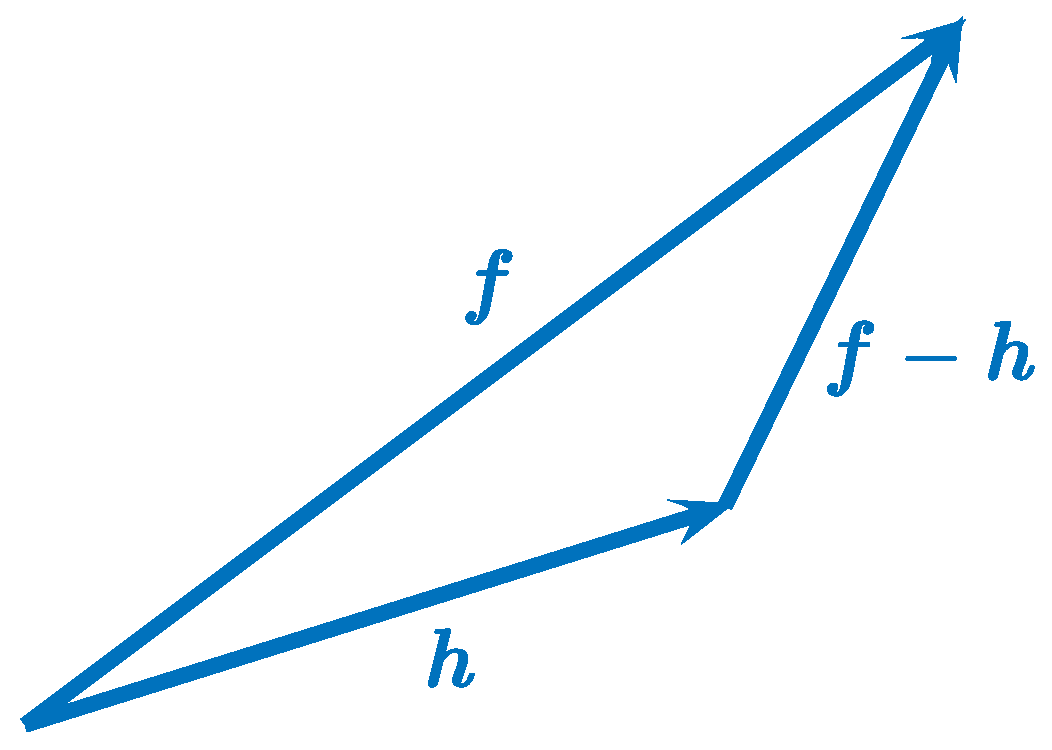
\includegraphics[width=\textwidth]{ProgramsImages/fhfmh.eps}
     \end{center}}\only<2>{How we \alert{should} think about $\ip{f}{h}$ for arbitrary vectors spaces $V$, e.g., spaces of functions.
 
 \medskip
 
Inner product comes first:  $\ip{\cdot}{\cdot \cdot} :  V \times V \to \reals$ satisfying
 \vspace{-1.5ex}
 \begin{gather*}
 \ip{0}{0} =0, \quad \ip{f}{f} > 0 \; \forall f \ne 0, \quad
 \ip{f}{h} =\ip{h}{f} \\
  \ip{cf+h}{k} = c \ip{f}{k} + c\ip{h}{k} 
 \end{gather*}

\vspace{-1.5ex}
Then distance and cosine
\vspace{-1.5ex}
 \begin{align*}
 	\norm{f} & := \sqrt{\ip{f}{f}}
 	\\
 	\cos(\measuredangle(f,h)) & : = \frac{\ip{f}{h}}{\norm{f}\norm{h}}  \\
 	& \in [-1,1] \text{ by Cauchy-Schwartz \hyperlink{CSProof}{\beamergotobutton{Proof}}}
  \end{align*}
 
 \vspace{-1.5ex}
 Law of cosines follows 

}
\end{column}
\end{columns}

\end{frame}

%%%%%%%%%%%%%%%%%%%%%%%%%%%%%%%%%%%%%%%%%%
%%%%%%%%%%%%%%%%%%%%%%%%%%%%%%%%%%%%%%%%%%
\section{Riesz Rep Thm for Hilbert Spaces}
%%%%%%%%%%%%%%%%%%%%%%%%%%%%%%%%%%%%%%%%%%
%%%%%%%%%%%%%%%%%%%%%%%%%%%%%%%%%%%%%%%%%%

\begin{frame}[label = generalRiesz]{Riesz Representation Theorem for a Hilbert Space $(V,\ip{\cdot}{\cdot})$}
	
	\vspace{-1ex}
\begin{theorem}[Riesz Representation Theorem for Hilbert Spaces] 
    If $\LIN: V \to \reals$ is any \alert{continuous} linear real-valued function on the \alert{Hilbert space} $(V,\ip{\cdot}{\cdot})$, then there \alert{exists a unique} $g \in V$, dependent on $\LIN$, for which $\LIN(f) =  \ip{g}{f}$ for all $f \in V$.
\end{theorem}
\only<1>{
\vspace{-5ex}
\begin{align*}
    \text{Hilbert space} & = \text{a vector space that is \alert{complete} under } \norm{\cdot}  \\
    & \qquad \text{(sequences that should converge  do)} \\
    & \qquad \text{may be \alert{infinite} dimensional $=$ no finite basis} \\
    \text{continuous } & \text{means } \sup_{f \in V} \frac{\abs{\LIN(f)}}{\norm{f}} < \infty \text{ (automatic for finite dimensional $V$)}
\end{align*}

Can we prove this theorem \alert{without referring to a basis} for $V$?}
\only<2->{\begin{proof}
\alert{Existence.} \only<2-5>{Define $\ker(\LIN) = \{f \in V : \LIN(f) = 0\}$ as the \only<2>{ $\dim(V) - 1$ dimensional }subspace of $V$ that $\LIN$ maps into $0$. \only<2>{If $\ker(\LIN) = V$, then all vectors in $V$ are mapped to $0$ and $g = 0$.}\only<3->{$\ker(\LIN) = V$ is easy.  Otherwise, pick any nonzero $g_\perp \in \{ h \in V : \ip{h}{f} = 0 \ \forall f \in \ker(\LIN)\}$ \hyperlink{lemma}{\beamergotobutton{How?}}, i.e., $g_\perp$ is orthogonal to all vectors in $\ker(\LIN)$.  \uncover<4->{ For any $f \in V$, let $h = \LIN(f) g_\perp - \LIN(g_\perp)f$, and note that}}

\only<3->{\vspace{-3ex}}
\begin{tabular}{m{0.7\textwidth}m{0.3\textwidth}}
\uncover<4->{\[
\begin{aligned}
\LIN(h) & = \LIN\bigl(\LIN(f) g_\perp - \LIN(g_\perp)f \bigr) \\
& = \LIN(f)\LIN(g_\perp) - \LIN(g_\perp)\LIN(f) = 0, 
\end{aligned}
\]

\vspace{-1.5ex}
so $h \in \ker(\LIN)$.  \uncover<5->{The choice of $g_\perp$ implies that
\vspace{-1.5ex}
\begin{gather*}
0 = \ip{g_\perp}{h} = \LIN(f)\ip{g_\perp}{g_\perp}  - \LIN(g_\perp) \ip{g_\perp}{f}, \quad \\
\LIN(f) = \frac{\LIN(g_\perp)\ip{g_\perp}{f}}{\ip{g_\perp}{g_\perp}} = \ip{g}{f} \quad \text{for } g:= \frac{\LIN(g_\perp)g_\perp}{\norm{g}^2}.
\end{gather*}}}
&
\includegraphics<2>[width = 0.25\textwidth]{ProgramsImages/kernelLinear.eps}
\includegraphics<3>[width = 0.25\textwidth]{ProgramsImages/kernelgperp.eps}
\includegraphics<4->[width = 0.25\textwidth]{ProgramsImages/RieszRepThm.eps}
\end{tabular}
}
\only<6->{Done.
	
\alert{Uniqueness.} Same proof as before.} \qedhere
\end{proof}}
    
\end{frame}




\begin{frame}{What Can We Do with the Riesz Representation Theorem?}
	
	\vspace{-1ex}
	
\begin{theorem}[\only<4>{Preliminary }Error Bound for Numerical Integration] 
	Let $(V,\ip{\cdot}{\cdot})$ be a Hilbert space of functions on $[0,1]^d$.  Suppose that integration and function evaluation are both continuous, linear real-valued functions on $V$.  Then the error of approximating the integral of a function in $V$ by the sample mean is
		\[
    	\abs{\int_{[0,1]^d} f(\vx) \, \dif \vx - \frac 1n \sum_{i=1}^n f(\vx_i) }
    				= \abs{\ip{\eta}{f}} = \abs{\cos\bigl(\measuredangle(\eta,f) \bigr)} \norm{\eta} \norm{f} 
    				\le \norm{\eta} \norm{f} \qquad \forall f \in V,
		\]
		for some  $\eta \in V$ that depends on $\vx_1, \ldots, \vx_n$, but not on $f$.

	\end{theorem}
	
	\vspace{-1ex}
\only<1,4>{\alert{Significance}
	
	\vspace{-2ex}

\begin{itemize}
	\item Error bound separates the $f$ dependent part from the algorithm dependent part ($\eta$)
	
	\item Algorithm developers can concentrate on 
	
	\item  Providential if  $\eta$ is nearly orthogonal to $f$ \cite{Hic17a}
	
	\item<4> \alert{How to find $\eta$?}
\end{itemize}}
\only<2,3>{\begin{proof}
		Note that 
		$
		\INT : f \mapsto \int_{[0,1]^d} f(\vx) \, \dif \vx \quad$ and $\AVG: f \mapsto \frac 1n \sum_{i=1}^n f(\vx_i)
		$
		 are continuous, linear real-valued functions.  \only<3->{Thus, so is $\ERR = \INT - \AVG$.  By the Reisz Representation Theorem, there exists an $\eta \in V$ such that
		 $
		 \int_{[0,1]^d} f(\vx) \, \dif \vx - \frac 1n \sum_{i=1}^n f(\vx_i)  = \ERR(f) = \ip{\eta}{f}
		 $.}
	\end{proof}}
\end{frame}

%%%%%%%%%%%%%%%%%%%%%%%%%%%%%%%%%%%%%%%%%%
%%%%%%%%%%%%%%%%%%%%%%%%%%%%%%%%%%%%%%%%%%
\section{Reproducing Kernels}
%%%%%%%%%%%%%%%%%%%%%%%%%%%%%%%%%%%%%%%%%%
%%%%%%%%%%%%%%%%%%%%%%%%%%%%%%%%%%%%%%%%%%

\begin{frame}{Reproducing Kernels \cite{Aro50}}
	Suppose that  $(V,\ip{\cdot}{\cdot})$  is  Hilbert space of functions on $\Omega$ for which function evaluation is a continuous, linear functional.  Then there exists, $K: \Omega \times \Omega \to \reals$ called a \alert{reproducing kernel} for which 
	\begin{equation*}
		\underbrace{K(\vt,\vx) = K(\vx,\vt)}_{\text{symmetry}},  \quad \underbrace{K(\cdot,\vx) \in V}_{\text{belonging}}, \quad  \underbrace{f(\vx) = \ip{K(\cdot,\vx)}{f}}_{\text{reproduction}}  \qquad \forall \vt, \vx \in \Omega, \; f \in V
	\end{equation*}
\uncover<2->{Combining with the Riesz Reproduction Theorem
\begin{gather*}
	\ERR(f) := \int_{[0,1]^d} f(\vx) \, \dif \vx - \frac 1n \sum_{i=1}^n f(\vx_i) 
	= \ip{\eta}{f}, \qquad \eta = ?\\
	\eta(\vx) = \ip{K(\cdot,\vx)}{\eta} =  \ip{\eta}{K(\cdot,\vx)} = \ERR\bigl(K(\cdot,\vx)\bigr) 
	\uncover<3->{= \int_{[0,1]^d} K(\vt,\vx) \, \dif \vt- \frac 1n \sum_{i=1}^n K(\vx_i,\vx) \\
		\uncover<4->{\norm{\eta}^2 = \ip{\eta}{\eta} = \ERR(\eta) 
			\uncover<5->{= \int_{[0,1]^{2d}} K(\vt,\vx) \, \dif \vt \, \dif \vx
				-  \frac 2n \sum_{i=1}^n \int_{[0,1]^d} K(\vx_i,\vx)  \, \dif \vx 
				+  \frac 1{n^2} \sum_{i,j=1}^n K(\vx_i,\vx_j)
			}
		}
	}
\end{gather*}
}
\end{frame}


\begin{frame}{Putting It Together}
	
	\vspace{-2ex}
	
	\begin{theorem}[Error Bound for Numerical Integration] 
		Let $(V,\ip{\cdot}{\cdot})$ be a Hilbert space of functions on $[0,1]^d$ with reproducing kernel, $K$.  Suppose that integration and function evaluation are both continuous, linear real-valued functions on $V$.  Then the error of approximating the integral of a function in $V$ by the sample mean is
		\[
		\abs{\int_{[0,1]^d} f(\vx) \, \dif \vx - \frac 1n \sum_{i=1}^n f(\vx_i) }
		\le \BAD(\vx_1, \ldots, \vx_n) \BAD(f),
		\]
		where 
		\begin{gather*}
			\BAD^2(\vx_1, \ldots, \vx_n) =  \int_{[0,1]^{2d}} K(\vt,\vx) \, \dif \vt \, \dif \vx
			-  \frac 2n \sum_{i=1}^n \int_{[0,1]^d} K(\vx_i,\vx)  \, \dif \vx 
			+  \frac 1{n^2} \sum_{i,j=1}^n K(\vx_i,\vx_j) ,\\
			\BAD(f) = \norm{f}.
		\end{gather*}
		
	\end{theorem}
	
\end{frame}

\finalthanksnote{These slides are  available at \\  \href{https://speakerdeck.com/fjhickernell/quasi-monte-carlo-software}{\nolinkurl{speakerdeck.com/fjhickernell/quasi-monte-carlo-software}}\\
	Google Colaboratory notebook at \href{https://tinyurl.com/QMCPyTutorial}{\nolinkurl{tinyurl.com/QMCPyTutorial}}\\
	Blog at \href{https://qmcpy.wordpress.com/}{\nolinkurl{qmcpy.wordpress.com/}}}


\thankyouframe

\begin{frame}{References}
    \printbibliography
\end{frame}





%%%%%%%%%%%%%%%%%%%%%%%%%%%%%%%%%%%%%%%%%%
%%%%%%%%%%%%%%%%%%%%%%%%%%%%%%%%%%%%%%%%%%
\section{Deleted Scenes}
%%%%%%%%%%%%%%%%%%%%%%%%%%%%%%%%%%%%%%%%%%
%%%%%%%%%%%%%%%%%%%%%%%%%%%%%%%%%%%%%%%%%%



\begin{frame}[label = CSProof]{Proof of the Cauchy-Schwarz Inequality \hyperlink{dotproduct}{\beamerreturnbutton{Back}}}
	
	\begin{theorem}[Cauchy-Schwarz] Let $(V,\ip{\cdot}{\cdot})$ be a real-valued inner product space.  Then
		\begin{equation}\tag{C-S} \label{eq:C-S}
		\abs{\ip{f}{h}} \le \norm{f} \norm{h} \qquad \forall f, h \in V,
		\end{equation}
		with equality iff $c_1 f + c_2 h = 0$ for some nonzero $(c_1, c_2)$.
	\end{theorem}

\only<1>{\begin{proof}[Proof of Inequality]
	If $f$ or $h$ are zero, the inequality becomes an equality by direct calculation.  For any nonzero $f, h \in V$, define the quadratic polynomial $p$ as follows:
		\begin{equation*}
			p(t) :=  \norm{t f + h}^2 = \ip{t f + h}{t f + h} = t^2 \ip{f}{f} + 2t \ip{f}{h} + \ip{h}{h} 
			= t^2 \norm{f}^2 + 2t \ip{f}{h} + \norm{h}^2.
		\end{equation*} 
		Since $p(t) \ge 0$ by definition, $p$ cannot have two roots, which means that  $\bigl(\ip{f}{h}\bigr)^2 - \norm{f}^2 \norm{h}^2$ must be non-positive.  This implies the inequality for $\abs{\ip{f}{h}}$. 
\end{proof}}
\only<2->{\begin{proof}[Proof of Equality]
		Recall that
		\begin{equation*}
			p(t) :=  \norm{t f + h}^2
			= t^2 \norm{f}^2 + 2t \ip{f}{h} + \norm{h}^2.
		\end{equation*} 
		Equality in \eqref{eq:C-S} happens iff $\abs{\ip{f}{h}} = \norm{f} \norm{h}$, which implies that $p$ has a single root, $t_0$.  Then
		\[
		0 = p(t_0) = \norm{t_0 f + h}^2,
		\]
		which is true iff $t_0 f + h = 0$ by the definition of a norm. 
\end{proof}}
	
\end{frame}
%\end{document}

\begin{frame}[label = lemma]{There Exists a Nonzero $g_\perp$ Orthogonal to All of $\ker(V)$ \hyperlink{generalRiesz}{\beamerreturnbutton{Back}}}
\vspace{-0.5ex}
	\begin{lemma}
		If $\LIN: V \to \reals$ is any \alert{continuous}, linear functional on the Hilbert space $(V,\ip{\cdot}{\cdot})$, and $\ker(\LIN) := \LIN^{-1}(\{0\}) = \{f \in V : \LIN(f) = 0\} \ne V$,
		then there exists a nonzero $g_\perp \in \{ h \in V : \ip{h}{f} = 0 \ \forall f \in \ker(\LIN)\}$.
	\end{lemma}
	\vspace{-1ex}
	\begin{proof}
	\only<1>{	Define $\dist\bigl(h,\ker(\LIN)\bigr) := \inf\{ \norm{h - f} : f \in \ker(\LIN)\}$, i.e., the closest $\ker(\LIN)$ comes to $h$.  For any $h \notin \ker(\LIN)$, choose $k_n \in \ker(\LIN)$ such that $\norm{h - k_n}^2 \le \dist^2\bigl(h,\ker(\LIN)\bigr) + 1/n$ for $n = 1, 2, \ldots$.  By the \alert{parallelogram law}, 
		
		\vspace{-3.5ex}
		\begin{align*}
			\norm{k_m - k_n}^2 &= \norm{(k_m - h) - (k_n-h) }^2 = 2\norm{k_m - h}^2 + 2\norm{k_n-h}^2 - \norm{(k_m - h) + (k_n-h) }^2 \\
			&= 2\norm{k_m - h}^2 + 2\norm{k_n-h}^2 - 4\norm{(k_m+k_n)/2-h) }^2 \qquad (k_m+k_n)/2 \in \ker(\LIN))\\
			& \le 2\bigl[\dist^2\bigl(h,\ker(\LIN)\bigr) + 1/m] + 2\bigl[\dist^2\bigl(h,\ker(\LIN)\bigr) + 1/n] \\
			&\qquad \qquad - 4\dist^2\bigl(h,\ker(\LIN)\bigr) = 2(1/m+1/n)
		\end{align*}
		
		\vspace{-2ex}
		So, $k_n \to k \in V$ due to \alert{completeness} of $V$; $k \in \ker(\LIN)$ due to continuity of $\LIN$.
		
		\vspace{-1.5ex}
		\[
		\norm{h-k} = \lim_{n \to \infty} \norm{h-k_n} =  \lim_{n \to \infty} \sqrt{\dist^2\bigl(h,\ker(\LIN)\bigr) + 1/n} = \dist\bigl(h,\ker(\LIN)\bigr)
		\]
		}%
		\only<2->{Let $g_\perp = h-k$.  Since $h \notin \ker(\LIN)$ and $k \in \ker(\LIN)$, then $h\ne k$ and 
		\[
		\norm{g_\perp} = \norm{h-k} = \dist\bigl(h,\ker(\LIN)\bigr) \ne 0.
		\]
		Pick any $f \in \ker(\LIN)$, and note that $k + tf \in \ker(\LIN)$ for all $t \in \reals$.  Thus,
 		\begin{align*}
 		\norm{g_\perp}^2 &\le \norm{h - (k+ tf)}^2 = \norm{g_\perp -tf}^2 
 		= \norm{g_\perp}^2 - 2t \ip{g_\perp}{f} + t^2 \norm{f}^2\\
 		0 & \le t \bigl[ -2\ip{g_\perp}{f} + t \norm{f}^2 \bigr] \qquad \forall t \in \reals
 		\end{align*}
 		The only way to ensure this inequality for all $t$ is for $\ip{g_\perp}{f} = 0$.
		\qedhere}
	\end{proof}
\end{frame}


\end{document}




\begin{frame}{Riesz Representation Theorem for $\reals^d$, Alternative Proof}
\begin{theorem}
    If $\LIN: \reals^d \to \reals$ is any linear functional, and $\ip{\vf}{\vh} : = \vf^T \vh$, then there exists a unique $\vg \in \reals^d$, dependent on $\LIN$, for which $\LIN(\vf) =  \ip{\vg}{\vf}$ for all $\vf \in \reals^d$
\end{theorem}
\begin{proof}
\alert{Existence.} Let $\mK$ be the $d$-dimensional identity matrix and let $\vK_j \in \reals^d$ denote its $j^{\text{th}}$ column.  Note that 
\[
f_j = \ip{\vK_j}{\vf} \qquad \forall \vf \in \reals^d.
\]
Now define $\vg \in \reals^d$ by $g_j = \LIN(\vK_j)$.
Then for all $\vf = (f_1, \ldots, f_d)^T$,
    \begin{align*}
    \LIN(\vf) &= L\bigl( \ve_1 f_1 + \cdots + \ve_d f_d \bigr)  = \LIN(\ve_1) f_1 + \cdots + \LIN(\ve_d) f_d \qquad \text{by linearlity} \\
    & = \ip{\vg}{\vf}, \qquad \text{where } \vg = \bigl( \LIN(\ve_1), \ldots, \LIN(\ve_d) \bigr)^T
    \end{align*}
\alert{Uniqueness.} If $\LIN(\vf) =  \ip{\vg}{\vf} =  \ip{\tvg}{\vf}$ for all $\vf \in \reals^d$, then 
\[
0 = \LIN(\vg - \tvg) - \LIN(\vg - \tvg)= \ip{\vg}{\vg - \tvg} - \ip{\tvg}{\vg - \tvg} = \ip{\vg - \tvg}{\vg - \tvg} = \norm{\vg - \tvg}^2
\]
so $\vg - \tvg = \vzero$ and $\vg = \tvg$.
\end{proof}
    
\end{frame}

